\chapter{位形空间}
\problem{定性画出沿着操场跑道跑步时你的世界线, 并分析其与跑道的关系.}
\begin{solution}
    世界线在每一时刻与该时刻的位形空间交于一点, 所有这样的点的集合即在跑道上跑步的轨迹. 该路径是位形空间中的一条封闭曲线.
\end{solution}

\problem{如图\ref{fig:2-2}所示, 两个粒子由一条无质量、不可拉伸的软绳连接, 绳长为$l$. 粒子$m_2$放在固定的水平面上, 绳子穿过水平面上的小孔, 另一端悬挂粒子$m_1$.
不考虑摩擦, 假设$m_2$可以在整个水平面上运动, $m_1$只在竖直方向运动. 
\begin{enumerate}[label=(\arabic*)]
    \item 分析这两个粒子和绳子构成的系统的位形和约束, 给出约束方程, 并分析约束是否完整、定常约束;
    \item 求系统的自由度.
\end{enumerate}}
\begin{figure}[h]
    \centering
    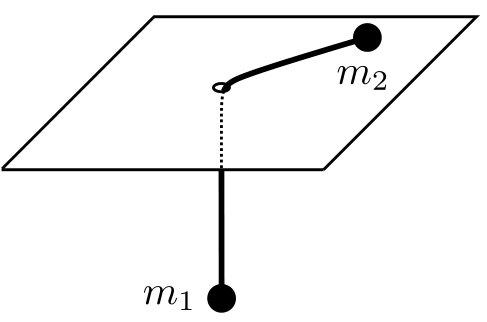
\includegraphics[width=0.3\textwidth]{content/Figures/2-2}
    \caption{ }
    \label{fig:2-2}
\end{figure}
\begin{solution}
    \begin{enumerate}[label=(\arabic*)]
        \item 设无约束时的广义坐标为$\{r_1, r_2, \theta\}$, 其中$r_1$和$r_2$分别是粒子与小孔之间的距离, $\theta$是粒子$m_2$在平面上运动的角度.
        约束方程为\[
            \phi (r_1, r_2, \theta) = r_1 + r_2 - l = 0
        \]
        注意到该约束方程是广义坐标的函数, 因此为完整约束; 且不显含时间, 因此为定常约束.
        \item 完整约束可减少一个自由度, 因此系统的自由度为$2$, 即最少只需两个独立的广义坐标$\{r, \theta\}$即可完全描述粒子的位形.
    \end{enumerate}
\end{solution}

\problem{如图\ref{fig:2-3}所示, 质量为$M$的楔块放在水平面上, 斜角分别为$\theta_1$和$\theta_2$, 底边长$L$. 两个质量分别为$m_1$和$m_2$的粒子, 
由一根无质量、不可拉伸的软绳连接, 绳长为$l$, 两个粒子分别放在楔块的两个斜面上. 不考虑摩擦, 
\begin{enumerate}[label=(\arabic*)]
    \item 分析楔块、两个粒子以及绳子组成的系统的位形与约束, 给出约束方程, 并分析约束是否完整、定常约束;
    \item 求系统的自由度.
\end{enumerate}}
\begin{figure}[h]
    \centering
    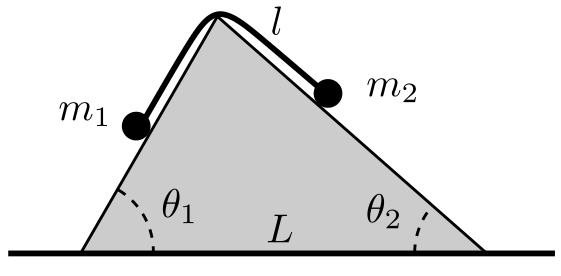
\includegraphics[width=0.3\textwidth]{content/Figures/2-3}
    \caption{ }
    \label{fig:2-3}
\end{figure}
\begin{solution}
    待施工.
\end{solution}
